\documentclass[a4paper,10pt]{article}
%\usepackage[latin1]{inputenc} % Paquetes de idioma
\usepackage[utf8]{inputenc} % Paquetes de idioma
\usepackage[spanish]{babel} % Paquetes de idioma
\usepackage{graphicx} % Paquete para ingresar gráficos
\usepackage{grffile}
\usepackage{hyperref}
\usepackage{fancybox}
\usepackage{amsmath}
\usepackage{amsfonts}
\usepackage{listings}
\usepackage{enumerate}
\usepackage{csquotes}
\usepackage{longtable}
\usepackage{pdflscape}
\usepackage{comment}

\usepackage[a5paper,hmargin=3cm,vmargin=5cm]{geometry}
\usepackage{lipsum,graphicx}
\usepackage[absolute]{textpos}
\usepackage{fancyhdr}
\usepackage{typearea}
\fancypagestyle{lscape}{%
  \fancyhf{}
  \fancyhead[L]{%
    \tikz[remember picture,overlay]
      \node[outer sep=1cm,below,rotate=90] at (current page.west) 
      {\textsf{Facultad de Ingenier\'ia $-$ Universidad de Buenos Aires}};}
      
  \fancyhead[R]{%
    \tikz[remember picture,overlay]
\node[outer sep=1.5cm,below,rotate=90] at (current page.west) {\textsf{PROYECTO
 DE TESIS DE INGENIERÍA INFORMÁTICA}                                \thepage};}
  \fancyfoot[R]{%
    \tikz[remember picture,overlay]
      \node[outer sep=2cm,above,rotate=90] at (current page.east) {\textsf{Estudiante: Soler, Francisco}};}




\renewcommand{\headrulewidth}{0pt}
\renewcommand{\footrulewidth}{0pt}

}

% Paquetes de macros de Circuitos
%\usepackage{pstricks}
\usepackage{tikz}
\usepackage[colorinlistoftodos,prependcaption,textsize=tiny]{todonotes}

\usepackage{tabto}

\newcommand{\personalData}[2]{%
  \textbf{\indent #1 \NumTabs{6}\tab\tab{#2}}\\%
}

% Encabezado y Pié de página
\usepackage{fancyhdr} % Paquete para encabezados y pie de página
\pagestyle{fancy} % Sin esta línea no se imprimiría el encabezado en todas las páginas

\fancyhf{} %  Borra el encabezado anterior (Por defecto escribe el títutlo de la sección en la que se encuentra la hoja
\setlength{\headheight}{22.55pt}
\fancyhead[L]{
	{\textsf{Facultad de Ingenier\'ia $-$ Universidad de Buenos Aires \\ PROYECTO DE TESIS DE INGENIERÍA INFORMÁTICA}}
}
%\addtocounter{page}{5}
\fancyhead[R]{\thepage}

\renewcommand{\footrulewidth}{0.4pt} % Ajusta el tamaño de las líneas separadoras en el pié de página
\renewcommand{\headrulewidth}{0.4pt} % Ajusta el tamaño de las líneas separadoras en el encabezado

\fancyfoot[L]{
	{\textsf{Trabajo Pr\'actico N$^{\circ}3$}: Etapas con Transistores Integrados} \\
	{\textsf{Integrantes: Torres Feyuk, Soler, Pastorino}}
	}
		

% Carátula del Trabajo
\title{ \author{} % Lo pongo para que el warning no moleste :p
\setlength{\unitlength}{1cm} %  Especifica la unidad de trabajo
\thispagestyle{empty}

\begin{picture}(18,0)
\put(0,0){
\includegraphics[width=1.5cm, height=3cm]{Logo1.png}}

\put(10.5,0){
\includegraphics[width=3cm, height=3cm]{Logo2.png}}

\end{picture}
\\[1.5cm]
\begin{center}
	\textbf{{\Huge Facultad de Ingenier\'ia \\ Universidad de Buenos Aires}}\\[2cm]
	{PROYECTO DE TESIS DE INGENIERÍA INFORMÁTICA}\\[0.5cm]
	{Calibración de una antena polarimétrica utilizando los acoplamientos 
	mutuos}\\[2.5cm]
\end{center}

\begin{flushleft}
	\textbf{ESTUDIANTE:}  Soler, Jos\'e Francisco \\[0.5cm]
	\textbf{PADR\'ON:} 91227 \\[0.5cm]
	\textbf{COORDINADORES:} Ing. Marino, Pablo - Ing. Wachenchauzer, Rosita\\[0.5cm]
\end{flushleft}
\date{} % Hace que no se imprima la fecha en la cual se compilo el .tex
 }

\begin{document}
	\maketitle % Hace que el título anterior sea el principal del documento
	
	\tableofcontents % Esta línea genera un indice a partir de las secciones y 
					 % subsecciones creadas en el documento
	\newpage

	\section{INTRODUCCIÓN}
    
Las antenas de arreglo de fase controlada [\ref{sarAntenna}] son utilizadas en 
aplicaciones de todo tipo, por ejemplo comunicaciones de móviles 
[\ref{ppr:mutual-ext1}], aéreas [\ref{ppr:punc-ext1}] y espaciales 
[\ref{ppr:dist1}][\ref{ppr:classic8}]. 

Para generar diversos productos, por ejemplo imágenes satelitales en radares de
apertura sintética [\ref{ppr:puncTrgt1}], 
es necesario que estén correctamente calibradas [\ref{ppr:classic1}] 
[\ref{ppr:classic2}][\ref{ppr:classic3}]. Esto implica, que las tolerancias de
fases y amplitudes se mantengan en el tiempo y/o sus valores sean bien conocidas
para cada elemento del arreglo.

Generalmente, este tipo de antenas son calibradas en tierra utilizando fuentes 
externas de campo lejano o cercano [\ref{ppr:mutual1}]. Sin embargo, en 
aplicaciones aéreas o espaciales, la utilización de dichas fuentes es impráctica
o difícil de implementar [\ref{ppr:mutual3}]. Resulta fundamental un esquema de
calibración interna que permita tener bajo control estas variables. Generalmente
se implementan lazos de calibración internos [\ref{ppr:classic1}]
[\ref{ppr:classic2}][\ref{ppr:classic3}][\ref{ppr:abs-rad-ical1}]
[\ref{ppr:classic4}][\ref{ppr:classic5}][\ref{ppr:classic6}]
[\ref{ppr:classic-ext1}][\ref{ppr:classic7}][\ref{ppr:classic8}]. 
Luego se opta por caracterizar todos aquellos componentes que no entran dentro 
de dicho lazo de calibración [\ref{ppr:abs-rad-ical1}].
Este método presenta algunos inconvenientes. Por dar un par de ejmplos se puede
mencionar que los recursos necesarios (tiempo, personal) durante la campaña de 
ensayos previa al lanzamiento impactan en todo el desarrollo de actividades, o
que las consecuencias que puede traer el hecho de que la caracterización no sea
válida porque un determinado componente envejece con el paso del tiempo.

En este contexto, se investiga y propone un método que permita reducir costos 
asociados a la calibración y por ende a los proyectos:

\begin{enumerate}
    \item Evitando la necesidad de realizar caracterizaciones previas de la 
antena de arreglo de fase.
    \item Permitiendo conocer en tiempo real, y para el estado real de la antena
, los valores reales de fase y amplitud en vuelo que transmite la antena, 
independientemente de su estado de envejecimiento.
\end{enumerate}

En este sentido se investiga y aprovecha el concepto acoplamiento mutuo 
inherente entre los módulos radiantes de la antena [\ref{ppr:mutual3}], pero de
manera complementaria al enfoque tradicional. 

En esta tesis se realizarán las siguientes tareas:

\begin{enumerate}
    \item Se explicarán las ventajas y desventajas del método propuesto respecto
del tradicional.
    \item Se analizarán y propondorán los requerimientos para poder 
implementarlo.
    \item Se desarrollará un modelo de antena de arreglo de fase polarimétrico 
básico representativo en parámetros S \ref{pr:parameters}.
    \item Se añadirán al mismo parámetros de dispersión de comportamiento que 
permitan analizar su comportamiento.
    \item Se realizará un modelo de calibración que será implementado 
algoritimicamente.
\end{enumerate}

\subsection{DEFINICIÓN}

{\textbf{Antena de arreglo de fase}} (en inglés: phased array) es un conjunto de
antenas en que las fases relativas de las señales con que se alimenta cada 
antena se varían intencionadamente con objeto de alterar el diagrama de 
radiación del conjunto. Lo normal es reforzar la radiación en una dirección 
concreta y suprimirla en direcciones indeseadas. Si todos los elementos del 
arrreglo de fase están contenidos en el mismo plano y la señal con que se 
alimentan es de la misma fase, entonces se estará reforzando la dirección 
perpendicular a ese plano. Si se altera la fase relativa de las señales se podrá
 \enquote*{mover} el haz (en realidad lo que se está haciendo es cambiar la 
dirección en la cual las interferencias son constructivas). Se consigue de este
modo hacer barridos sin necesidad de movimiento físico, con la ventaja añadida
de que se pueden barrer ángulos del orden de miles de grados por segundo. Esto
permite utilizar la antena para compaginar simultáneamente funciones de 
detección y de seguimiento muchos blancos individuales, asi como para obtener 
imágenes de apertura sintética. Su uso se va extendiendo debido a la 
confiabilidad derivada del hecho de que no tienen partes móviles. Casi todos los
radares militares modernos se basan en phased arrays, relegando los sistemas 
basados en antenas rotatorias a aplicaciones donde el costo es un factor 
determinante (tráfico aéreo, meteorología, etc) Su uso está también extendido en
aeronaves militares debido a su capacidad de seguir múltiples objetivos. El 
primer avión en usar uno fue el B-1B Lancer, y el primer caza, el MiG-31 ruso.\\

{\textbf{Calibración interna}} es colocar sensores que permitan la medición 
directa u indirecta de los distintos parámetros del sistema en vuelo. 

Estas mediciones obtenidas con este sistema son útiles solamente al utilizarlas
en conjuto a los resultados de los test realizados en tierra, los cuales definen
la relación entre lo observado y la performance de los párametros del sistema. 
Ejemplos de satélites para los cuales se utilizó calibración interna son el 
E-ERS-1 y el SIR-C.
    
Los tests realizados en tierra para dichos sistemas complejos son sobre la
electrónica de RF, la electrónica digital y la antena sobre temperatura; para 
los cuales es preferible realizarlos, cuando sea posible, en un ambiente al 
vacío. Los parámetros clave del sistema, como: potencia transmitida, pérdidas de
transmisión o recepción, ganancia de recepción, ganancia y patrón de la antena, 
linealidad de la electrónica digital/RF, rango dinámico, y fase/amplitud vs 
estabilidad de la frecuencia son medidos en función de la temperatura para cada 
seteo de ganancia del radar y PRF (Pulse Repetition Frequency). Los elementos de
calibración, como medidores de temperatura, de corriente y de potencia, podrán 
permitir la determinación de la performance del sistema en función de la 
variación de dichos parámetros.
    
Esta técnica asume que la variación en la performance del sistema puede ser 
modelada en función de los parámetros observables. También, se asume que los 
componentes de calibración están correctamente calibrados y son estables en el 
paso del tiempo. Además de estos tests, en la mayoría de los sistemas de radar 
se realizan mediciones de componentes de RF utilizando loops de calibración.
		
\section{MOTIVACIÓN}

A la hora de adquirir imágenes satelitales es crucial que se conozca 
perfectamente la señal emitida y recibida por la antena. Ya sea por 
envejecimiento de los componentes [\ref{ppr:mutual1}] o por variaciones de 
temperaturas se observan dispersiones de las mismas [\ref{ppr:sim1}]. 


El método de calibración tradicional, por lazos de calibración internos, permite
calibrar una antena de arreglo de fase, aunque adolece de algunos defectos entre
los cuales se incluyen:

\begin{enumerate}
    \item Una degradación o directamente rotura de un elemento radiante, el cual
está fuera del lazo de calibración interno, no es detectado por la calibración 
interna.
    \item Existen elementos que quedan fuera del lazo de calibración interno. 
Como por ejemplo los circuladores. Esto lleva a la necesidad de realizar 
caracterizaciones en tierra lo cual implica consumo de recursos de proyecto 
importantes, además de tener que confiar que dicha caracterización será válida 
(o sea que no habrá envejecimiento de los mismo) luego durante vuelo en toda la
vida útil de la antena.
    \item Cada lazo de calibración no se interrelaciona con el resto haciendo 
que no se pueda disminuir el error de medición por multiplicidad de caminos.
\end{enumerate}

Esto lleva a investigar opciones superadoras, que den lugar a un método de 
calibración que permita complementar al tradicional evitando la necesidad de 
realizar costosas caracterizaciones en tierra, previendo que los componentes en
vuelo puedan envejecer y por ende dichas caracterizaciones no ser más validas, 
permitiendo detectar fallas en elementos que en la calibración interna 
tradicional quedan fuera del lazo de calibración, y disminuyendo la 
incertidumbre en la determinación de la fase y amplitud de salida.

El método que se propone en esta tesis, denominado de \enquote*{método de 
calibración interna complementada por acoplamientos mutos (MCINCAM)} toma la 
idea de mediciones por acoplamiento mutuo [\ref{ppr:mutual1}][\ref{ppr:mutual2}]
[\ref{ppr:mutual3}][\ref{ppr:mutual-ext1}], para integrarla de manera 
complementaria al método tradicional, sin necesidad de agregar hardware 
adicional, y además establece los requerimientos electrónicos para poder 
implementarla. En esta tesis además se realiza un modelo ad hoc, en parámetros 
S, de antena, para mostrar la eficacia del método. 


\section{Objetivo de la tesis}

La presente tesis tiene varios objetivos:

\begin{enumerate}
    \item Presentar conceptualmente el método tradicional de calibración interna
de una antena polarimétrica que abarque el sistema completo de transmisión/
recepción. con sus virtudes y defectos. Mencionar algunas misiones de ejemplo en
las cuales el mismo se ha utilizado.
    \item Investigar, desarrollar y presentar conceptualmente un método 
alternativo de calibración interna que introduzca mejoras al método tradicional 
sin necesidad de introducir hardware adicional y con la premisa fundamental de 
reducir los costos asociados a las caracterizaciones que el método tradicional 
incluye. Introducir los requerimientos necesarios para poder implementarlo.
    \item Investigar, desarrollar y presentar (generar) los algoritmos que 
permitan representar el modelo de antena polarimétrico (modelo de capa física) 
que serán utilizados para poder comparar el método tradicional y el alternativo.
Dichos modelos deben representar el comportamiento en RF básico de las señales 
al propagarse por el sistema.
    \item Generar los algoritmos que permitan correr el algoritmo de calibración
alternativo de manera de poder comparar ambos métodos.
    \item Sacar conclusiones respecto a los pros y contras del método propuesto,
en particular en referencia al método tradicional, por medio de algunos 
parámetros objetivos como ser tiempo de calibración, caracterizaciones 
necesarias, incertidumbre de medición, entre otros.
\end{enumerate}    


\section{Especificaciones del problema}

\begin{itemize}
    \item La aplicación debera reproducir el comportamiento en RF de los 
elementos individuales: cables, psc, TRM, elementos radiantes.

    \item La aplicación deberá reproducir el comportamiento del sistema el cual 
será LTI (lineal e invariante en el tiempo).
    
    \item La antena debe estar compuesta por defasadores, atenuadores, cables, 
divisores de potencia y módulos radiantes.
    
    \item Se deben poder utilizar distintos divisores/combinadores de potencia. 
La diferencia entre ellos es la cantidad de puertos de salida.
    
    \item Los componentes de la antena deben caracterizarse utilizando 
parámetros de alta frecuencia.
    
    \item Se debe tener en cuenta el efecto que impone un componente al resto de
la antena.

    \item Se debe poder configurar la dimensión de la antena.
    \item Se debe poder configurar la distancia entre elementos radiantes.
    \item Se debe poder configurar los atributos que afecten la modelización de
cada componente de la antena. 
    
    \item Se debe poder configurar el largo de los cables.
    \item Se debe poder configurar la atenuación de los cables.
    
    \item Se debe poder configurar el error de comportamiento de cada
componente de la antena de forma independiente.

    \item Se deben poder configurar los atenuadores y defasadores a la hora de 
realizar la calibración. 

    \item La aplicación debe poder calibrar una antena polarimétrica con el 
método de calibración convencional.
    
    \item La aplicación debe poder calibrar una antena polarimétrica con el
método de calibración alternativo.
    
    \item La aplicación debe poder calibrar la potencia de transmisión y 
recepción.
    
    \item La aplicación debe poder calibrar la fase de transmisión y 
recepción.
    
    \item La aplicación debe poder calibrar en ambas polarizaciones: horizontal
y vertical.
    
    \item Se debe poder alcanzar el estado de calibración deseado partiendo 
cualquier estado inicial en los defasadores y atenuadores.
    
    \item No se puede calibrar en la misma polarización transmisión y recepción 
a la vez.
    
    \item La antena tiene que ser perfectamente plana. No deben haber 
imperfecciones.
           
    \item Se debe poder configurar la frecuencia de trabajo.

    \item Se debe poder configurar los parámetros de error (desvío estandar) 
para la ganancia y fase de la chirp utilizada entre pulsos.

    \item Se debe poder configurar los parámetros de error (desvío estandar) 
para la ganancia y fase de la chirp réplica utilizada a la hora de realizar la 
calibración convencional.
    
    \item Se debe poder configurar los parámetros de error (desvío estandar) 
para la fase de la codificación utilizada a la hora de realizar la calibración
convencional.

    \item Se debe poder simular, configurar la destrucción total de elementos de
la antena SAR como ser los TRMs.
\end{itemize}


\section{Metodología de la tesis}

		En la presente tesis se investigarán los métodos de calibraciones 
	actuales para poder determinar que ventajas, desventajas, limitaciones y 
	diferencias hay entre cada una de ellos. Se buscará tener una visión global
	de esta problemática para poder determinar y entender que posibles falencias
	puede tener este método alternativo.

		Posteriormente, se investigarán las limitaciones que poseen las antenas 
	polarimétricas para poder determinar que recaudos se deben tener en cuenta a
	la hora de desarrollar el método.

		Luego, tomando todo en cuenta, se determinarán las hipótesis necesarias
	para que el algoritmo funcione correctamente. Para la validación del método
	se realizará un modelo de antena.
		
		Finalmente, se probarán, analizarán y documentarán los resultados 
	obtenidos de la comparación entre el algoritmo propuesto y el algoritmo de
	la calibración convencional. A su vez, se dejará asentado que posibles 
	mejoras se podrían aplicar al algoritmo para determinar otros aspectos que
	están fuera del alcance de esta tesis.


\section{Estado de Situación}
		La calibración de una antena polarimétrica se ha estudiado en numerosas 
	ocasiones, abordando el problema desde distintos enfoques. A continuación se
    pueden observar los distintos métodos utilizados, clasificados por la 
    utilización o no de componentes externos.

	\[
		\substack{\text{métodos}\\de\\\text{calibración}}
		\begin{cases}
			\substack{\text{utilizan}\\\text{componentes externos}}
			\begin{cases}
				
				\text{blancos puntuales - [\ref{ppr:puncTrgt1}], 
				[\ref{ppr:puncTrgt2}], [\ref{ppr:punc-ext1}], 
				[\ref{ppr:puncTrgt3}]}\\
				\text{blancos distribuidos - [\ref{ppr:dist1}]}\\
				\text{absolute Radiometric Calibration - [\ref{ppr:absRad1}],
				[\ref{ppr:rad2}], [\ref{ppr:rad3}], [\ref{ppr:abs-rad-ical1}], 
				[\ref{ppr:rad4}], [\ref{ppr:rad5}], [\ref{ppr:rad6}], 
				[\ref{ppr:rad7}]}\\
				\text{Broadcast Reference Technique - [\ref{ppr:brdcast1}]}\\
				\text{miden deformación antena - [\ref{ppr:aligment1}], 
				[\ref{ppr:aligment2}], [\ref{ppr:aligment3}], 
				[\ref{ppr:aligment4}], [\ref{ppr:aligment5}],
				[\ref{ppr:aligment6}]}\\
				\text{utilizan calibración externa - [\ref{ppr:ext1}], 
				[\ref{ppr:ext2}], [\ref{ppr:ext3}], [\ref{ppr:punc-ext1}], 
				[\ref{ppr:classic-ext1}], [\ref{ppr:mutual-ext1}]}\\
			\end{cases}\\
			\substack{\text{no utilizan}\\\text{componentes externos}}
			\begin{cases}
				\text{calibración clásica - [\ref{ppr:classic1}], 
				[\ref{ppr:classic2}], [\ref{ppr:classic3}], 
				[\ref{ppr:abs-rad-ical1}], [\ref{ppr:classic4}], 
				[\ref{ppr:classic5}], [\ref{ppr:classic6}],
				[\ref{ppr:classic-ext1}], [\ref{ppr:classic7}],
				[\ref{ppr:classic8}]}\\
				\text{aprovechando acoplamiento mutuo - [\ref{ppr:mutual1}], 
                [\ref{ppr:mutual2}], [\ref{ppr:mutual3}], 
                [\ref{ppr:mutual-ext1}]}\\
				\text{método REV - [\ref{ppr:rev1}]}
			\end{cases}
		\end{cases}
	\]


La calibración interna es el método típicamente más utilizado pero adolece de 
algunos defectos como ser que:

\begin{itemize}
    \item Los circuladores no están incluidos dentro de dicho lazo de 
calibración interna. Esto obliga a que los mismos tengan que ser caracterizados
previamente y asegurar la estabilidad a lo largo de toda la vida útil de la
misión.
    \item Las antenas, o modulos radiantes, también quedan fuera del lazo de
calibración. Por ende, un módulo radiante que pudiese resultar dañado en vuelo,
no es detectable por el lazo interno de calibración.
    \item Durante los ensayos, se adolece de puntos de testeo que permitan 
corroborar que la potencia de salida por el modulo radiante es la esperada. No
hay acopladores direccionales entre el TRM y el modulo radiante entonces no es
posible si no es con un equipo de campo cercano poder ver la potencia de salida
de cada módulo radiante y la fase.
    \item Es necesario realizar una caracterización de la RFDN en temperatura lo
cual insume numerosos recursos y queda sujeto además a la suposición de que nada
cambien en el tiempo.
    \item Existe una incertidumbre dada reductible hasta cierto punto en la 
determinación de fase y amplitud de salida dada por lo que determina la cadena y
el camino en cuestión.
\end{itemize}

Por este motivo la calibración interna requiere de un método que complemente 
todos estos aspectos, mejorandolos. Es decir un método que:

\begin{itemize}
    \item Incorpore los circuladores al lazo de calibración interno (LCI).
    \item Incorpore los módulos radiantes al LCI.
    \item Permita durante los ensayos poder estimar la potencia real y fase con
la que emite cada uno de los módulos radiante sin la necesidad de incorporar
elementos adicionales como ser acopladoes direccionales.
    \item Evite o minimice las caracterizaciones previas que demandan una
cantidad de recursos para nada despreciable y que encarece las campañas.
    \item Permita minimizar la incertidumbre de salida en fase y ganancia.
\end{itemize}

Entre la biliografia de antenas existe un método denominado de calibración por 
acoplamiento mutuo, ver [\ref{ppr:mutual1}], [\ref{ppr:mutual2}], 
[\ref{ppr:mutual3}], [\ref{ppr:mutual-ext1}]. Este método no puede determinar la
 potencia y fase absoluta de transmisión de cada módulo radiante, solamente la 
potencia y fase relativa entre los mismos. Por ende, este método no es completo.

Se propone utilizar el método de acoplamiento mutuo como “complemento” del 
existente denominándolo método de “autocalibracion interna extendida”. Como 
ventaja, no solo se abarca todo el sistema sino que también es fácilmente 
implementable con el hardware ya existente. 

%\newgeometry{hmargin=3cm,vmargin=5cm}
%\thispagestyle{lscape}
%\begin{landscape}
 
    \section{Cronograma}
	
\begin{figure}[!htb]
 \centering
 %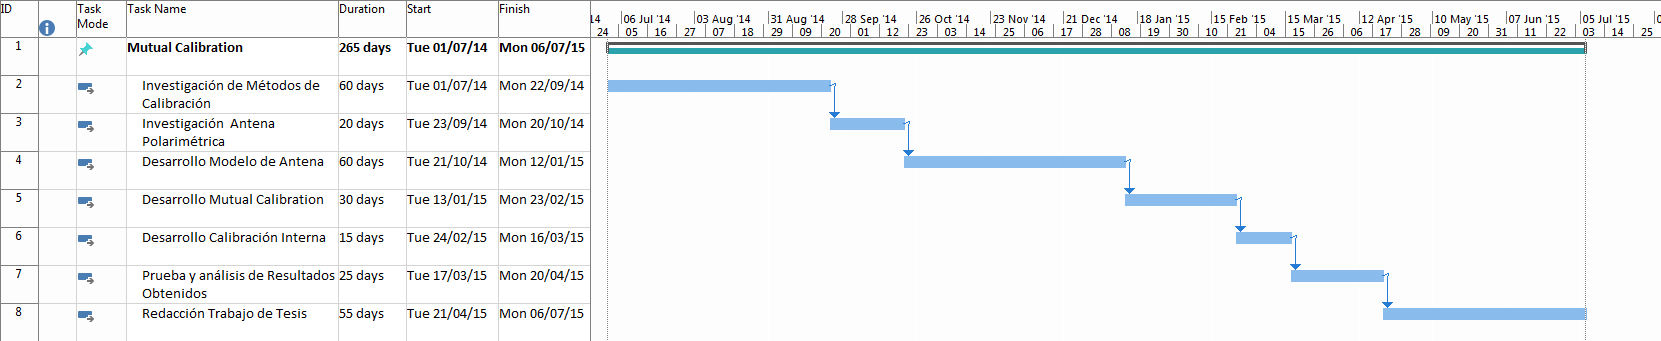
\includegraphics[width=1.5\textwidth]{Imagenes/CronogramaTesis.png}
 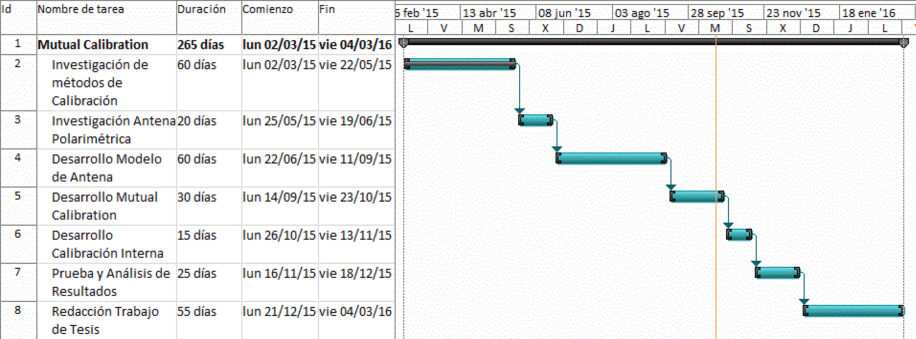
\includegraphics[width=\textwidth]{Imagenes/crono.png}
 \caption{Cronograma}
 \label{fig:crono}
\end{figure}

%    \end{landscape}
%\restoregeometry
       
    \subsection{Cronograma detallado}

En el cronograma se propone un tiempo de cuatro horas por día de trabajo, por lo tanto, las tareas quedan divididas de la siguiente forma:

\begin{itemize}
    \item 240 horas para investigar sobre los distintos métodos de calibración existentes.
    \item 80 horas para investigar sobre el funcionamiento de una antena polarimétrica.
    \item 240 horas para desarrollar un modelo de antena polarimétrica
    \item 120 horas para desarrolar la simulación del método de mutual Calibration.
    \item 60 horas para desarrollar la simulación del método de calibración interna.
    \item 100 horas para definir ensayar testear y extraer conclusiones de las 
comparaciones entre ambos métodos de calibración.
    \item 220 horas para redactar la tesis
\end{itemize}

	\newpage
	\section{Bibliografía}
	
	\begin{enumerate}[ {[}1{]} ]
		\item \label{ppr:aligment1} F. K. LI, \enquote*{A Method for Detection 
		of Deformations in Large Phased Array Antennas for Spaceborne Synthetic
		Aperture Radars}, IEEE TRANSACTIONS ON ANTENNAS AND PROPAGATION, VOL. 
		AP-32, NO. 5 , MAY 1984.
		
		\item \label{ppr:aligment2} G. M. Shaw and R. B. Dybdal, \enquote*{A 
		Space-Fed Local Oscillator for Spaceborne Phased Arrays}, 1988 IEEE 
		MTT-S Digest.

		\item \label{ppr:brdcast1} EU-AN LEE and C. NELSON DORNY, \enquote*{A 
		Broadcast Reference Technique for Self-calibrating of Large Antenna 
		Phased Arrays}, IEEE TRANSACTIONS ON ANTENNAS AND PROPAGATION, VOL. 37,
		NO. 8, AUGUST 1989.
		
		\item \label{ppr:classic1} Anthony P. Luscombe, \enquote*{Internal 
		Calibration Of The Radarsat Synthetic Aperture Radar}, Geoscience and 
		Remote Sensing Symposium, 1990. IGARSS'90. 'Remote Sensing Science for 
		the Nineties.
		
		\item \label{ppr:absRad1} L. M. H. Ulander, R. K. Hawkins, C. E.
		Livingstone and T . I. Lukowski, \enquote*{Absolute Radiometric 
		Calibration of the CCRS SAR}, IEEE TRANSACTIONS ON GEOSCIENCE AND REMOTE
		SENSING, VOL. 29. NO. 6. NOVEMBER 1991.
		
		\item \label{ppr:puncTrgt1} Anthony Freeman, \enquote*{SAR Calibration: 
		An Overview}, IEEE Transactions on Geoscience And Remote Sensing, Vol. 
		30, NO. 6, November 1992.
		
		\item \label{ppr:rad2} H. LAUR, P. MEADOWS, J.I. SANCHEZ, E. DWYER, 
		\enquote*{ERS-1 SAR RADIOMETRIC CALIBRATION}, Published in the 
		Proceedings of the CEOS SAR Calibration Workshop (ESA WPP-048) Sept. 93
		
		\item \label{ppr:classic2} M. Zink, \enquote*{CALIBRATION AND 
		PERFORMANCE ANALYSIS OF THE X-SAR SYSTEM}, Geoscience and Remote Sensing
		Syposium, 1994. IGARSS 1994.
		
		\item \label{ppr:classic3} Jorgen Dall, Niels Skou, Erik Lintz 
		Christensen, \enquote*{Pulse-Based Internal Calibration of Polarimetric
		SAR}, Geoscience and Remote Sensing Syposium, 1994. IGARSS 1994.

		\item \label{ppr:rad3} Brian L. Markhaml, Suraiya P. Ahmadz, James R. 
		Irons1 and Darrel L. Williams1 \enquote*{Radiometric Calibration of the
		Landsat-7 Enhanced Thematic Mapper Plus}, Geoscience and Remote Sensing
		Syposium, 1994. IGARSS 1994.
		
		\item \label{ppr:dist1} Masanobu Shimada and Anthony Freeman, \enquote*{
		A Technique for Measurement of Spaceborne SAR Antenna Patterns Using 
		Distributed Targets}, IEEE TRANSACTIONS ON GEOSCIENCE AND REMOTE 
		SENSING, VOL. 33, NO. I , JANUARY 1995.
		
		\item \label{ppr:abs-rad-ical1}Anthony Freeman, M. Alves, B. Chapman, J.
		Cruz, Y. Kim, S. Shaffer, J. Sun, E. Turner, and Kamal Sarabandi, 
		\enquote*{SIR-C Data Quality and Calibration Results}, IEEE TRANSACTIONS
		ON GEOSCIENCE AND REMOTE SENSING, VOL. 33, NO. 4, JULY 1995.
		
		\item \label{ppr:mutual1} Ashok Agrawal and Allan Jablon, \enquote*{A 
		CALIBRATION TECHNIQUE FOR ACTIVE PHASED ARRAY ANTENNAS}, Phased Array 
		Systems and Technology, 2003, IEEE International Symposium.
		
		\item \label{ppr:puncTrgt2} David Stevens, Peter Bird, Gordon Keyte, 
		\enquote*{A SAR antenna calibration method}, Geoscience and Remote 
		Sensing Syposium, 1996. IGARSS 1996.
		
		\item \label{ppr:rev1} Uoshihisa Hara, Chikako Ohno, Masafumi Iwamoto, 
		and Natsuki Kondo, \enquote*{A Study on Radiometric Calibration of Next
		Generation Spaceborne SAR}, Geoscience and Remote Sensing Syposium, 
		1997. IGARSS 1997.

		\item \label{ppr:ext1} Seth D. Silverstein, \enquote*{Algorithms for 
		Remote Calibration of Active Phased Array Antennas for Communication 
		Satellites}, Signals, Systems and Computers, 1996.
		
		\item \label{ppr:ext2} J . M . Ashe, W . Yang, T. Shen, G. Xu and S. D.
		Silverstein, \enquote*{Experimental Study of Remote Calibration 
		Algorithms for Active Phased Array Transmitters}, Signals, Systems and
		Computers, 1996.
		
		\item \label{ppr:ext3} Daniel S. Purdy, \enquote*{In Orbit Active Array
		Calibration for NASA’s LightSAR}, Radar Conference, 1999. The Record of
		the 1999 IEEE.
		
		\item \label{ppr:punc-ext1} Hong Jun, Zang Bing-rong, Wing Hong-qi, 
		\enquote*{The progress of the aiirborne SAR calibration techniques in 
		China}, Geoscience and Remote Sensing Syposium, 1989. IGARSS 1989.

		\item \label{ppr:mutual2} Charles Shipley and Don Woods \enquote*{MUTUAL
		COUPLING-BASED CALIBRATION OF PHASED ARRAY ANTENNAS}, Phased Array 
		Systems and Technology, 2000. Proceedings. 2000 IEEE International 
		Conference.
		
		\item \label{ppr:rad4} Jeffrey A. Mendenhall, \enquote*{Radiometric 
		Calibration and Flight Validation}, ALI Tech\_Trans-1 JAM 10/23/01.

		\item \label{ppr:rad5} Volker Kaltenborn, \enquote*{Intern Report: 
		Volker Kaltenborn}, Alaska SAR Facility (ASF).
		
		\item \label{ppr:classic4} D J Bibby \& A J Knight, \enquote*{A RF Model
		of an Active Array Antenna for a Spaceborne SAR}, Antennas and 
		Propagation, 2003. (ICAP 2003). Twelfth International Conference.
		
		\item \label{ppr:classic5} Daniel Bast, \enquote*{Parameters Affecting 
		Orthogonal SAR Transmit and Receive Module Calibration}, European Space
		and Technology Centre, European Space Agency EOP-FI, Keplerlaan-1, 2200
		AG Noordwijk (The Netherlands).
		
		\item \label{ppr:puncTrgt3} M. Shimada, T. Tadono, and M. Matsuoka,
		\enquote*{Calibration and Validation of PALSAR}, Geoscience and Remote 
		Sensing Syposium, 2002. IGARSS 2002.
		
		\item \label{ppr:rad6} Kai-Jen Calvin Tien, Roger D. de Roo, \enquote*{
		Comparsion of Different Microwave Radiometric Calibration Techniques}, 
		Geoscience and Remote Sensing Syposium, 2004. IGARSS 2004.
		
		\item \label{ppr:aligment3} P. Zulch, R. Hancock, and J. McKay, 
		\enquote*{Array Deformation Performance Impacts on a LEO L-Band GMTI 
		SBR} 0-7803-8870-4/05/\$20.00© 2005 IEEE. IEEEAC paper \#1532, Version 
		5, Updated December 20, 2004.

		\item \label{ppr:classic6} A. G. Stove, \enquote*{ISSUES FOR THE 
		AUTOCALIBRATION OF PHASED ARRAY RADARS}, $1^{st}$ EMRS DTC Technical 
		Conference – Edinburgh 2004.
		
		\item \label{ppr:aligment4} J. J. M de Wit, W. L. van Rossum, M. P. G. 
		Otten, A. G. P. Koekenberg \enquote*{Concept for Measuring and 
		Compensating Array Deformation}, Proceedings of the 4th European Radar 
		Conference.
		
		\item \label{ppr:rad7} Marco Schwerdt, Benjamin Bräutigam, Markus 
		Bachmann, Björn Döring \enquote*{TerraSAR-X Calibration - First Results}

		\item \label{ppr:classic-ext1} S. K. Srivastava, N. W. Shepherd, T. I. 
		Lukowski and R. K. Hawkins \enquote*{PLANS FOR RADARSAT IMAGE DATA
		CALIBRATION}, Adv. Space Res. Vol. 17, No. 1, pp (1)89-(1)96, 1996.

		\item \label{ppr:aligment5} Elena Zaitsev, John Hoffman, \enquote*{
		Phased Array Flatness Effects on Antenna System Performance}, 978-1-4244
		-5128-9/10/\$26.00 \copyright 2010 IEEE

		\item \label{ppr:classic7} Shuo Wang, Haiming Qi, and Weidong Yu 
		\enquote*{An Internal Calibration Scheme for Polarimetric Synthetic 
		Aperture Radar System}, IEEE transactions on geoscience and remote 
		sensing, vol. 49, NO. 1, January 2011.
		
		\item \label{ppr:mutual-ext1} Wei Chen, Joni Polili Lie, Boon Poh Ng, 
		Tao Wang and Meng Hwa Er \enquote*{Joint Gain/Phase and Mutual Coupling
		Array Calibration Technique with Single Calibrating Source}, Hindawi 
		Publishing Corporation International Journal of Antennas and Propagation
		Volume 2012, Article ID 625165.

		%\item N. Fistas and A. Manikas \enquote*{A NEW GENERAL GLOBAL ARRAY 
		%CALIBRATION METHOD}, ICASSP PROCEEDINGS, APRIL 94.
		
		\item \label{ppr:classic8} Eduardo Makhoul, Antoni Broquetas, 
		Francisco López-Dekker, Josep Closa, and Paula Saameno \enquote*{
		Evaluation of the Internal Calibration Methodologies for Spaceborne 
		Synthetic Aperture Radars with Active Phased Array Antennas}, IEEE 
		JOURNAL OF SELECTED TOPICS IN APPLIED EARTH OBSERVATIONS AND REMOTE 
		SENSING, VOL. 5, NO. 3, JUNE 2012.

		\item \label{ppr:aligment6} Guillaume Lesueur, Daniel Caer, Thomas 
		Merlet, Pierre Granger \enquote*{Active compensation techniques for 
		deformable phased array antenna}, Thales Air Systems Hameau de Roussigny
		, 91470 Limours, France.

		\item \label{ppr:sim1} Will P. M. N. Keizer \enquote*{Fast and Accurate
        Array Calibration Using a Synthetic Array Approach}, IEEE TRANSACTIONS 
        ON ANTENNAS AND PROPAGATION, VOL. 59, NO. 11, NOVEMBER 2011.

		\item \label{ppr:mutual3} HERBERT M. AUMANN, ALAN J. FENN, FRANK G. 
        WILLWERTH \enquote*{Phased Array Antenna Calibration and Pattern 
        Prediction Using Mutual Coupling Measurements}, IEEE TRANSACTIONS ON 
        ANTENNAS AND PROPAGATION, VOL 31. NO 7 , JULY 1989.

        \item \label{sarAntenna} Alan J. Fenn, Donald H. Temme, William P. 
        Delaney, and William E. Courtney \enquote*{The Development of 
        Phased-Array Radar Technology}, VOLUME 12, NUMBER 2, 2000 LINCOLN 
        LABORATORY JOURNAL.
        
        \item \label{pr:parameters} F. Caspers. \enquote*{RF engineering basic 
concepts: S parameters}, CERN, Genova, Switzerland
	\end{enumerate}

	\newpage
	\section{Currículum Vitae}
	

\subsection*{Datos Personales}
\personalData{}{}
\personalData{Nombre: José Francisco Soler}{D.N.I.: 34765654}
\personalData{Domicilio: Adolfo Alsina 2550}{Capital Federal}
\personalData{Teléfono: 011-39041335}{}
\personalData{Fecha de nacimiento: 04/10/1989}{Edad: 26 años}
\personalData{Nacionalidad: Argentina}{Estado civil: soltero}	
\personalData{Mail: jose.francisco.tw@gmail.com}{}	

\subsection*{Formación Académica}
Escuela Provincial Técnica No 748, Trelew - Chubut: Egresado en el año 2007 con
honores. Orientación electrónica en Telecomunicaciones.

Facultad de Ingeniería, Universidad de Buenos Aires: Ingeniería en Informática e
Ingeniería en Electrónica. Aprobado Ciclo Básico Común; 240 créditos de un total
de 248, un promedio de 7.22 en Informática y 216 créditos en Electrónica.


\subsection*{Idiomas}
    Inglés, nivel upper intermediate.

\subsection*{Experiencia}
Ayudante en la materia Laboratorio desde el segundo cuatrimestre del 2010.
Realización de un trabajo práctico, el cual, constó del procesamiento de una 
señal en crudo, tomada con una antena de apertura sintética, en la materia 
Señales y Sistemas.

Análisis, diseño y construcción de un prototipo didáctico de sensor satelital. 
El cual consta de una plataforma con 8 sensores infrarrojos, dispuestos de tal 
forma que, colocando una maqueta con relieve, estos realizan un mapeo de la 
zona para luego mostrar por computadora el mapa topográfico resultante. Este 
prototipo se lo puede encontrar en las instalaciones de la escuela provincial 
de Trelew ex-enet No 748.

Trabajé en el negocio familiar en ventas durante 10 años.

Actualmente trabajando en CONAE en el área de sistemas, dedsde enero del 2014.

Manejo de Windows, Linux, Excel, Word, entre otros.

Lenguajes de programación: Pascal, C, C++, Java, Smalltalk, Oz, Go, Perl,
assembler, Python.

\newpage
	\section{Materias Aprobadas}	
	\begin{center}
		\scriptsize
		\centering
		\begin{longtable}{|p{3.5cm}|c|c|c|p{1.4cm}|c|c|}
			\hline 
			\bfseries Materia & \bfseries Fecha & \bfseries Resultado & 
			\bfseries Nota & \bfseries Forma de aprobación & \bfseries Acta & 
		 	\bfseries	Plan \\
			\hline
			(7801) IDIOMA INGLES & 29/06/2009 & Aprobado & 6 & Examen & 
			18-22-214 & 1986 \\
			\hline
			(6103) ANALISIS MATEMATICO II A & 13/08/2009 & Aprobado & 5 & Examen
			& 1-154-76 & 1986 \\
			\hline
			(7540) ALGORITMOS Y PROGRAMACION I & 18/08/2009 & Aprobado & 9 & 
			Examen & 17-101-183 & 1986 \\
			\hline
			(6201) FISICA I A & 18/08/2009 & Aprobado & 6 & Examen & 2-107-176 &
			1986 \\
			\hline
			(7541) ALGORITMOS Y PROGRAMACION II & 10/02/2010 & Aprobado & 8 & 
			Examen & 17-103-4 & 1986 \\
			\hline
			(6301) QUIMICA & 15/02/2010 & Aprobado & 6 & Examen & 3-75-25 & 1986
			\\
			\hline
			(6203) FISICA II A & 25/02/2010 & Aprobado & 8 & Examen & 2-108-63 &
			1986 \\
			\hline
			(6107) MATEMATICA DISCRETA & 02/03/2010 & Aprobado & 6 & Examen & 
			1-156-42 & 1986 \\
			\hline
			(7507) ALGORITMOS Y PROGRAMACION III & 06/07/2010 & Aprobado & 8 & 
			Examen & 17-104-12 & 1986 \\
			\hline
			(7531) TEORIA DE LENGUAJE & 07/07/2010 & Aprobado & 8 & Examen & 
			17-104-24 & 1986 \\
			\hline
			(6602) LABORATORIO & 12/07/2010 & Aprobado & 8 & Examen & 6-139-14 &
			1986 \\
			\hline
			(6108) ALGEBRA II A & 14/07/2010 & Aprobado & 8 & Examen & 1-153-219
			& 1986 \\
			\hline
			(6215) FISICA III D & 22/12/2010 & Aprobado & 8 & Examen & 2-108-221
			& 1986 \\
			\hline
			(6109) PROBABILIDAD Y ESTADISTICA B & 10/02/2011 & Aprobado & 8 & 
			Examen & 1-155-250 & 1986 \\
			\hline
			(6670) ESTRUCTURA DEL COMPUTADOR & 16/02/2011 & Aprobado & 7 & 
			Examen & 6-140-35 & 1986 \\
			\hline
			(6110) ANÁLISIS MATEMÁTICO III A & 24/02/2011 & Aprobado & 5 & 
			Examen & 1-157-49 & 1986 \\
			\hline
			(7512) ANALISIS NUMERICO I & 25/02/2011 & Aprobado & 8 & Examen & 
			17-106-55 & 1986 \\
			\hline
			(7542) TALLER DE PROGRAMACION I & 13/07/2011 & Aprobado & 10 & 
			Examen & 17-107-9 & 1986 \\
			\hline
			(7506) ORGANIZACION DE DATOS & 14/07/2011 & Aprobado & 5 & Examen & 
			17-107-17 & 1986 \\
			\hline
			(6620) ORGANIZACION DE COMPUTADORAS & 08/08/2011 & Aprobado & 8 & 
			Examen & 6-141-16 & 1986 \\
			\hline
			(7112) ESTRUCTURA DE LAS ORGANIZACIONES & 14/12/2011 & Aprobado & 4 
			& Examen & 11-153-84 & 1986 \\
			\hline
			(7114) MODELOS Y OPTIMIZACION I & 22/12/2011 & Aprobado & 6 & Examen
			& 11-153-145 & 1986 \\
			\hline
			(6211) MECANICA RACIONAL & 14/02/2012 & Aprobado & 8 & Examen & 
			2-109-191 & 1986 \\
			\hline
			(6606) ANALISIS DE CIRCUITOS & 15/02/2012 & Aprobado & 7 & Examen &
			6-141-176 & 1986 \\
			\hline
			(6674) SEÑALES Y SISTEMAS & 24/02/2012 & Aprobado & 8 & Examen & 
			6-141-206 & 1986 \\
			\hline
			(7508) SISTEMAS OPERATIVOS & 12/07/2012 & Aprobado & 7 & Examen & 
			17-109-103 & 1986 \\
			\hline
			(6609) LABORATORIO DE MICROCOMPUTADORAS & 13/07/2012 & Aprobado & 8
			& Examen & 6-142-46 & 1986 \\
			\hline
			(7509) ANALISIS DE LA INFORMACION & 13/08/2012 & Aprobado & 6 & 
			Examen & 17-110-54 & 1986 \\
			\hline
			(7552) TALLER DE PROGRAMACION II & 17/08/2012 & Aprobado & 10 & 
			Examen & 17-110-87 & 1986 \\
			\hline
			(7543) INTRODUCCIÓN A LOS SISTEMAS DISTRIBUIDOS	& 21/12/2012 & 
            Aprobado & 6 & Examen & 17-111-08 & 1986 \\
			\hline
			(7510) TECNICAS DE DISEÑO & 04/02/2013 & Aprobado & 6 & Examen & 
			17-111-36 & 1986 \\
			\hline
			(7515) BASE DE DATOS & 06/02/2013 & Aprobado & 8 & Examen & 
			17-111-44 & 1986 \\
			\hline
			(6608) CIRCUITOS ELECTRONICOS I & 27/02/2013 & Aprobado & 8 & Examen
			& 6-143-126 & 1986 \\
			\hline
			(7140) LEGISLACION Y EJERCICIO PROFESIONAL DE LA ING. EN INFORMÁTICA
			& 13/12/2013 & Aprobado & 8 & Examen & 71-0001453 & 1986 \\
			\hline
			(6618) TEORIA DE CONTROL I & 05/08/2013 & Aprobado & 6 & Examen & 
			86-0001220 & 1986 \\
			\hline
			(6675) PROCESOS ESTOCÁSTICOS & 09/08/2013 & Aprobado & 9 & Examen & 
			86-0001265 & 1986 \\
			\hline
			(7559) TECNICAS DE PROGRAMACION CONCURRENTE I & 13/08/2013 & 
			Aprobado & 8 & Examen & 95-0001370 & 1986 \\
			\hline
			(6669) CRIPTOGRAFIA Y SEGURIDAD INFORMATICA & 16/08/2013 & Aprobado
			& 8 & Examen & 86-0001295 & 1986 \\
			\hline
			(7567) SIST.AUTOM.DE DIAG.Y DETEC.DE FALLAS I & 04/08/2014 & 
			Aprobado & 7 & Examen & 95-0002261 & 1986 \\
			\hline
			(7565) MANUFACTURA INTEGRADA POR COMP.(CIM) I & 07/08/2014 & 
			Aprobado & 7 & Examen & 95-0002312 & 1986 \\
			\hline
			(7568) SIST.DE SOPORTE P/CELDAS DE PROD FLEXIB. & 10/12/2014 & 
			Aprobado & 10 & Examen & 95-0002440 & 1986 \\
			\hline
			(7566) MANUFACTURA INTEGRADA POR COMP.(CIM) II & 11/12/2014 & 
			Aprobado & 7 & Examen & 95-0002462 & 1986 \\
			\hline
			(6405) ESTATICA Y RESISTENCIA DE MATERIALES B & 15/12/2014 & 
			Aprobado & 9 & Examen & 64-0001589 & 1986 \\
			\hline
			(7201) MATERIALES INDUSTRIALES 1 & 05/03/2015 & 
			Aprobado & 8 & Examen & 72-0001442 & 1986 \\
			\hline
			\caption{Materias Aprobadas} \label{tab:matApr}
		\end{longtable}
	\end{center}
	
    \newpage
	\section{Plan de cursada}
	
	\begin{table}[!htb]
		\centering
		\begin{tabular}{|c|c|c|c|}
			\hline
			Código & Denominación & Créditos & Fecha \\
			\hline
			75.00 & TESIS & 24-OBL & 2 - 2015 \\
			\hline
		\end{tabular}
		\caption{Plan de cursada} \label{tabPlanCursada}
	\end{table}

	TOTAL CRÉDITOS: 24

\newpage
\begingroup
\pagestyle{empty}

\hfill Buenos Aires, 19 de Octubre de 2015

\noindent Sres

\noindent Comisión Curricular

\noindent Ingeniería en Informática
\\

Tenemos el agrado de dirigirnos a usted con el objeto de presentarle la 
propuesta de Tesis en Ingeniería en Informática del señor José Francisco Soler 
(Padrón 91227) que realizará bajo nuestra dirección.

Adjuntamos a la presente el Plan de tesis con su cronograma de desarrollo, el 
currículum del señor Soler y el listado de sus materias aprobadas, así como el 
acta-compromiso.

A la espera de su resolución los saluda atte.

\vspace*{3cm}

\hfill \parbox{4cm}{Lic. Rosa Wachenchauzer\\Directora} \hfill 
\parbox{3cm}{Ing. Pablo Marino\\Co Director}

\newpage

\section*{\centering Acta de Acuerdo para el Desarrollo de Tesis}

En Buenos Aires, a los diecinueve días del mes de octubre del año dos mil quince
se reúnen en el Departamento de Computación de la Facultad de Ingeniería de la 
Universidad de Buenos Aires la Lic. Rosa Wachenchauzer, el Ing. Pablo Marino y 
el alumno de la carrera Infeniería en Informática José Francisco Soler (91227) 
para dar tratamiento a la selección del Tema de Tesis y el Plan de Estudio 
Personal para el Ciclo Superior de la carrera.

Se acuerda establecer como Tema de Tesis de Grado de Ingeniería en Informática 
del señor Francisco Soler \textbf{\enquote*{Calibracion de una antena 
polarimétrica utilizando los acoplamientos mutuos}}.

El plan de Estudios Personal del señor Soler, de la orientación en SISTEMAS DE 
PRODUCCIÓN, comprende la cursada de las materias optativas SEÑALES Y SISTEMAS 
(66.74), ANÁLISIS DE CIRCUITOS (66.06), MATEMÁTICA DISCRETA (61.07) y TEORÍA DE 
CONTROL 1 (66.18), que abarcan los conocimientos suficientes para desarrollar 
satisfactoriamente la tesis de Grado.

Sin más que tratar se firman tres ejemplare de la presente acta, uno para elevar
a la Direccion del Departamento de Computación, otro para el estudiante y un 
tercero para el profesor.

\vspace*{3cm}

Francisco Soler \hfill \parbox{4cm}{Directora\\Lic. Rosa Wachenchauzer} \hfill
\parbox{3cm}{Co Director\\ Ing. Pablo Marino}

\clearpage
\endgroup
\end{document}
